% !TEX root = ./rosbook_jp.tex
%-------------------------------------------------------------------------------
\chapterimage{chapter_head_1.pdf}

%-------------------------------------------------------------------------------
\chapter{ROS入門}

%-------------------------------------------------------------------------------
\section{ロボットソフトウェアプラットフォーム}
\index{プラットフォーム}

1973年に発売された世界初の商用携帯電話Motorola DynaTAC  8000は、重量が0.8kgもあり、およそ携帯とは呼べないほど持ち運びに不便であった。しかし、現在のスマートフォンは、インターネット、SNS、メッセージ、ゲーム、音楽鑑賞など、さまざまな機能を備え、もはや日常生活に欠くことができない最も身近な機器となっている。
初期の携帯電話メーカーは、薄く軽量で、かつ長時間、高品質の通話を実現するために熾烈なハードウェア開発競争を繰り広げ、他社に先駆けて新しい機能を搭載した新製品を次々と投入した。また、新たな機器の性能を最大限に生かせるよう、特定の機種に対応したファームウェア(機器制御用基本ソフトウエア)を個別に開発していた。このため、新しいハードウェアが開発されるたびに、その開発スケジュールに合わせて新たにファームウェアを開発する必要があった。このようなハードウェアに重点を置いた開発は、ソフトウェア開発にかかる管理コストの増加をもたらし、開発スピードも徐々に低下していった。
この問題を解決するために、Android、iOS, Windows Phoneなど、特定のハードウェアに依存しないスマートフォン向けオペレーティングシステムが開発された。携帯電話メーカーはこれらを採用することで、管理コストを抑えつつ、新たな機能の追加が容易に行えるようになった。さらに、ハードウェアに精通していなくても関連アプリケーションが開発できるようになり、ハードウェアよりもソフトウェアにより重きを置いた「アプリ開発者」と呼ばれる新しい職種まで登場した。
以上のように、携帯電話およびスマートフォン市場の急成長は、2つの段階に分けられる。第1段階は、ハードウェアの発達と爆発的なユーザー数の増加に支えられていた。第2段階は、スマートフォン向けオペレーティングシステムの登場と、それによるアプリケーションの開発時間や管理コストの削減、開発者のすそ野の広がりに依るところが大きい。

%-------------------------------------------------------------------------------
\subsection{ロボットソフトウェアプラットフォームがもたらす変化}
\index{OSRF}

ロボット開発も、携帯電話やスマートフォンによく似た歴史を辿っている。従来、ロボット用アプリ開発者は、ロボットのハードウェア構成を強く意識した専用のソフトウェアを開発してきた。しかし、スマートフォンと同様に、汎用的なロボットオペレーティングシステム、あるいはソフトウェアプラットフォームが開発されれば、アプリ開発者はそこで動作するアプリケーション開発に資源を集中できる。ロボットソフトウェアプラットフォームは、スマートフォンの成長における初期の開発/発展段階にあり、少々乱立気味ともいえるほど多くの種類が発表されている。以下に、特に広く利用され、開発が盛んなロボットソフトウェアプラットフォームと、その開発母体を示す。\\
\\
\textbf{ロボットソフトウェアプラットフォームの例}
\begin{itemize}[leftmargin=*]
\item ERSP\footnote{\url{http://www.evolution.com/products/ersp/}}、Evolution Robotics
\item MSRDS\footnote{\url{http://msdn.microsoft.com/en-us/robotics/default.aspx}}、Microsoft
\item MARIE\footnote{\url{http://marie.sourceforge.net/}}、LABORIUS
\item URBI\footnote{\url{http://www.urbiforge.org/}}、Gostai\footnote{\url{http://www.gostai.com/}}
\item ROS\footnote{\url{http://www.ros.org/}}、Open Source Robotics Foundation\footnote{\url{http://www.osrfoundation.org/}} 、(OSRF、米国)
\item OpenRTM\footnote{\url{http://www.openrtm.org}}、産業技術総合研究所 (AIST、 日本)
\item OROCOS\footnote{\url{http://www.orocos.org/}}、KU Leuven、LASS、KTHなどのヨーロッパ連合(ヨーロッパ)
\item OPRoS\footnote{\url{http://www.opros.or.kr/}}、ETRI、KIST、KITECH、江原大学(韓国)
\item NAOqi\footnote{\url{https://www.aldebaran.com/ja/naoqi-os}}、ソフトバンク(日本)、Aldebaran(フランス)
\end{itemize}
\vspace{1\baselineskip}
このように、これまでに様々なロボットソフトウェアプラットフォームが開発されているが、その優劣を一概に論じることは難しい。なぜなら、使いやすいコンポーネントの追加機能や通信機能、可視化、シミュレータ、リアルタイム性など、各プラットフォームがそれぞれユニークな機能を提供しているからである。しかし、現在のパーソナルコンピュータのオペレーティングシステム(OS)のように、ロボットソフトウェアプラットフォームも、いずれは淘汰され、統合されていくと予想される。
本書は、OSRF(Open Source Robotics Foundation)により開発、メンテナンスが行われているROS(Robot Operating System)の解説書である。ROSは、上述した多くのロボットソフトウェアプラットフォームの中でも、ユーザー数、提供ライブラリの種類と数、拡張性の高さ、開発の容易さなどの点で特に優れている。ROSコミュニティは世界各地で活発に活動しており、ROSコミュニティが中心となりWeb上に蓄積された数多くの資料から、利用中に生じた疑問点や不具合の情報を容易に得ることができる。さらに、ROSはOSRFが単独で開発しているのではなく、大学の研究者、企業の開発者、趣味で活動するハーベスト(hobbyist)、さらにはロボットを専門とする人々だけでなく、コンピュータサイエンス、コンピュータビジョン、あるいは通信ネットワークの専門家など、多様な人々が開発に携わっている点で特徴的である。

%-------------------------------------------------------------------------------
\subsection{ロボットソフトウェアプラットフォームがもたらす未来}

ロボットソフトウェアプラットフォームを利用すると、ロボットのハードウェアに対する知識をそれほど持たなくても、ロボット用アプリケーションの開発が可能である。これは、最新のスマートフォンのハードウェア構成や詳細を知らなくとも、アプリを開発できることと同様である。
以前は、ロボット開発者、あるいはロボットメーカは、ハードウェアの設計からソフトウェア開発まで一貫して手掛けていた。しかし、ロボットソフトウェアプラットフォームに準拠すれば、ソフトウェアに精通した多様な人材がロボットアプリケーション開発に参加できる。一方、ハードウェア開発者は、ソフトウェアプラットフォームで提供するインターフェースに合わせてハードウェアを設計すればよい。これにより携帯電話と同様、ロボットメーカはアプリケーションの開発時間や管理コストを削減でき、ロボット分野が急速に発展するきっかけとなり得る。

%-------------------------------------------------------------------------------
\section{ROSとは}
\index{ROS}

ロボットソフトウェアプラットフォーム一般について理解したところで、ここからはROSについて説明する。まずは、そもそもROSとは何なのかを明らかにしよう。
ROSの公式サイトであるROS Wiki\footnote{\url{http://wiki.ros.org/ROS/Introduction}}では、ROSを以下のように定義している。

\begin{textbox}
ROS (Robot Operating System)はソフトウェア開発者のロボット・アプリケーション作成を支援するライブラリとツールを提供しています。具体的には、 ハードウェア抽象化、デバイスドライバ、ライブラリ、視覚化ツール、 メッセージ通信、パッケージ管理などが提供されています。
\end{textbox}

つまり、ROSは異なるハードウェアでも共通して使用できるロボットオペレーティングシステムであり、アプリケーション開発のための様々なツールを備えたソフトウェアプラットフォームである。

%-------------------------------------------------------------------------------
\subsection{ROSは新しいオペレーティングシステム(OS)か}
\index{Meta-Operating System}
\label{section:metaos}

オペレーティングシステムには、汎用コンピュータ向けのものとしてWindows(Windows 7、8、10 ...)、Linux(Ubuntu、Fedora、Gentoo ...)、MAC(OS X Yosemite、EL Capitan...)などがあり、スマートフォン向けのものとしてはAndroid、iOS、Symbian、RiMO、Tizenなどが有名である。Robot Operating Systemという名前から、特にROSに初めて接する読者は、ROSをこれらの汎用コンピュータ向けのオペレーティングシステムと同様なものと捉えているかもしない。しかし、より正確に表現すれば、ROSは図1-1に示すようなメタ・オペレーティングシステム(Meta-Operating System)である。メタ・オペレーティングシステムとは、オペレーティングシステム上で動作し、同一、あるいは異なるオペレーティングシステム(あるいはコンピュータ)で動作しているプロセスに対し、プロセス間通信やスケジューリング、負荷の監視、エラー処理などを支援するシステムである。つまり、ROSは、Windows、Linux、Androidに取って代わるロボットのためのオペレーティングシステムではなく、上記のオペレーティングシステムで動作するプロセスを制御するシステムである。
例えば、Linuxの頒布形態(ディストリビューション)であるUbuntu上で動作するROSは、Ubuntuのプロセス管理システム、ファイルシステム、ユーザインタフェース、プログラムユーティリティ(コンパイラ、スレッドモデルなど)などを利用している。ROSは、これに加えて様々なセンサやロボットなどのハードウェアの制御、プロセス間通信、スケジュール、エラー処理など、ロボットアプリケーションの開発に必要な機能をライブラリとして提供している。またROSは、ROSを利用して開発された様々なアプリケーションパッケージを管理し、流通する仕組み(生態系、Ecosystem)を備えている。
このようにROSとは、既存の伝統的なオペレーティングシステムを利用しながら、ロボットアプリケーションの開発に必須となるロボットやセンサの制御システムを、ハードウェア抽象化の概念に基づいてパッケージ化したものである。さらに様々なアプリケーションもパッケージとして提供することで、ユーザーによるロボットアプリケーション開発を強力に支援する。

\begin{figure}[h]
  \centering
  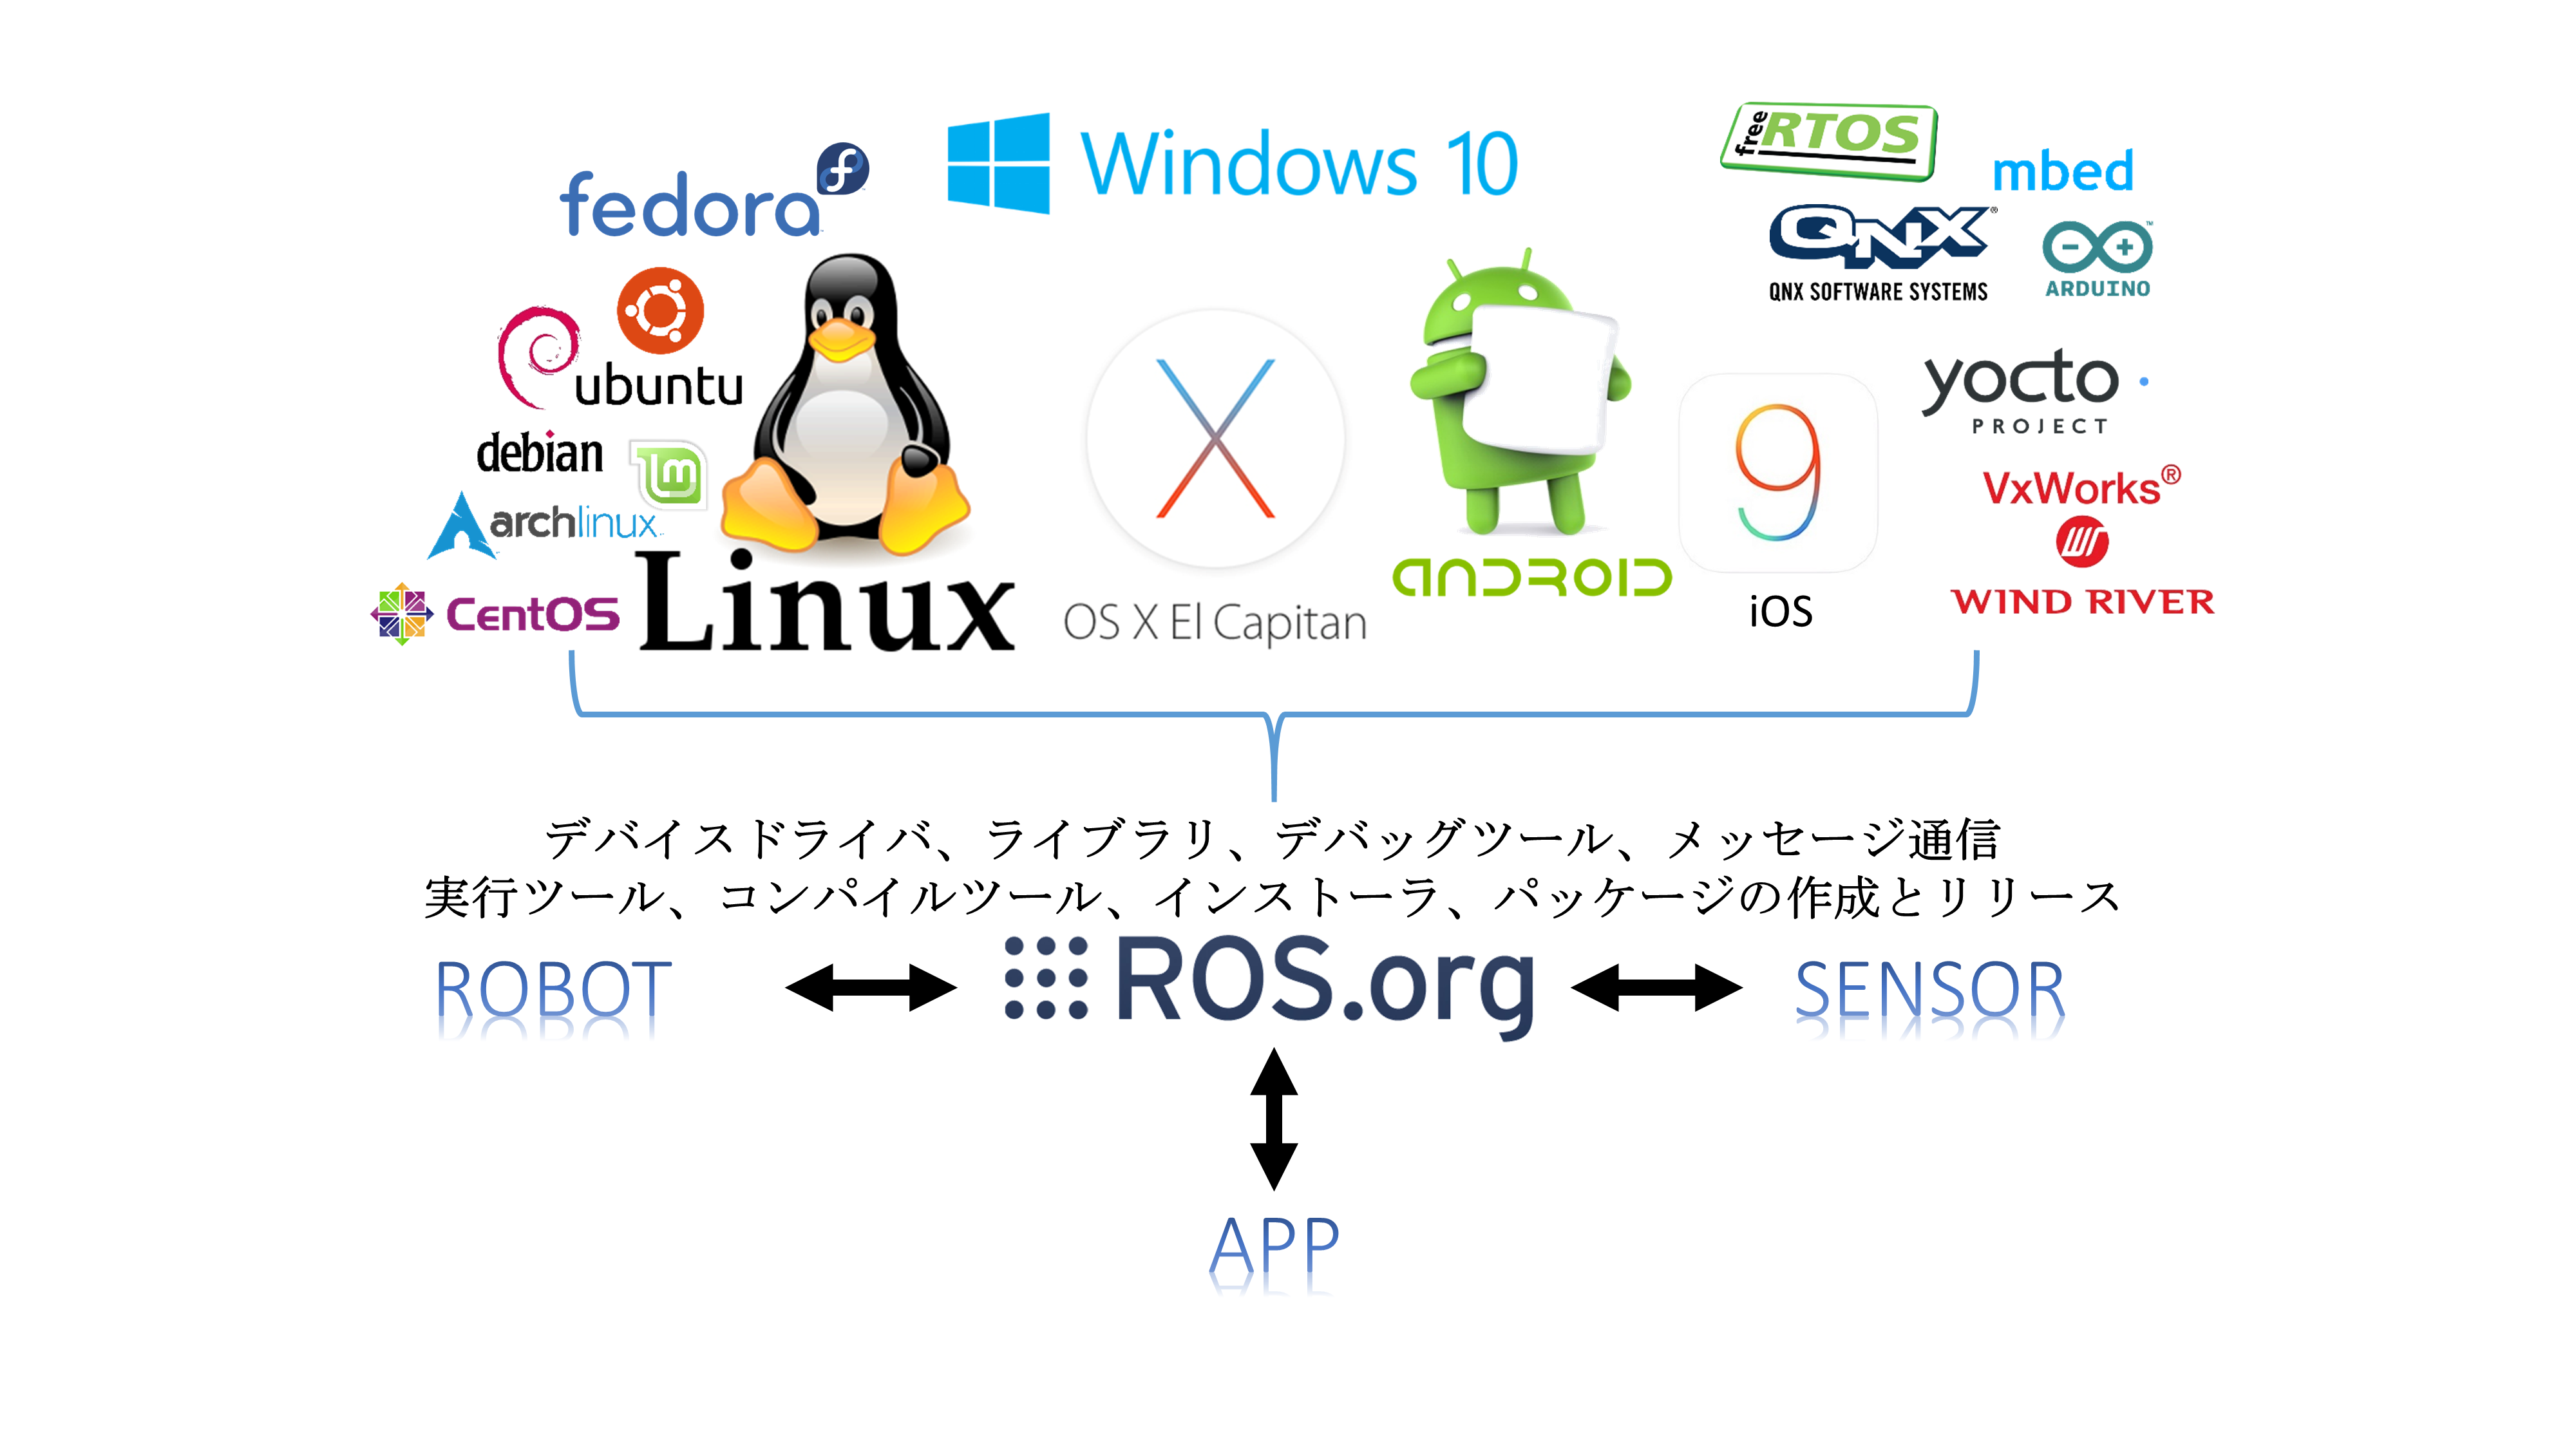
\includegraphics[width=\columnwidth]{pictures/chapter1/pic_01_01.png}
  \caption{メタ・オペレーティングシステムとしてのROS}
\end{figure}


また図1-2のように、ROSでプロセス間通信に使用されるメッセージは、異なるオペレーティングシステムや異なるハードウェア上のプロセス間でも自由に情報をやり取りすることができる。したがってROSは、様々なハードウェアから構成される複雑なロボットの開発にも適したオペレーティングシステムである。これについては、後半の章でより詳細に取り上げる。

\begin{figure}[h]
  \centering
  \includegraphics[width=\columnwidth]{pictures/chapter1/pic_01_02.png}
  \caption{異なるオペレーティングシステムやハードウェア上のプロセスに対する通信}
\end{figure}

%-------------------------------------------------------------------------------
\subsection{ROS生態系}
\index{生態系}\index{Ecosystem}

近年、Android、iOS、Symbian、RiMO、Tizenなどスマートフォン向けオペレーティングシステムの開発現場では、生態系(Ecosystem)、あるいはモバイル生態系という単語をよく耳にする。これは、スマートフォンの製造会社と販社、様々なアプリケーションを開発するサードパーティ、さらにユーザーが有機的に密に結びつけられたモデルのことである。例えば、スマートフォン製造会社がオペレーティングシステムで定められたインターフェースに合わせて機器を製造し、各オペレーティングシステム会社は、これに合わせたライブラリを作成して提供する。ソフトウェア開発者は提供されたライブラリを利用することで、ハードウェアの深い知識がなくても容易にサービスプログラムを開発できる。さらに、開発されたプログラムをユーザーが入手しやすいように流通させることで、収益が循環し、市場が成長する。この生態系には軸となるオペレーティングシステムが必要であり、パーソナルコンピュータ分野ではマイクロソフト社のWindows OSとフリーソフトウェアのLinuxがこれに当たる。
現在、ロボット分野でも同様の流れが見られる。つまり、当初は様々なハードウェアが乱立し、これらを統合するためのオペレーティングシステムが開発されていなかった。しかし現在では、様々なソフトウェアプラットフォームが提案され、特にROSはいち早く生態系の枠組みを整えつつある。今後、ロボット製造会社やセンサ製造会社などのロボット関連ハードウェアメーカー、およびROSの開発運用チームには、アプリ開発者やユーザーにも広く恩恵が及ぶようなROS生態系の確立が期待されている。

\begin{figure}[h]
  \centering
  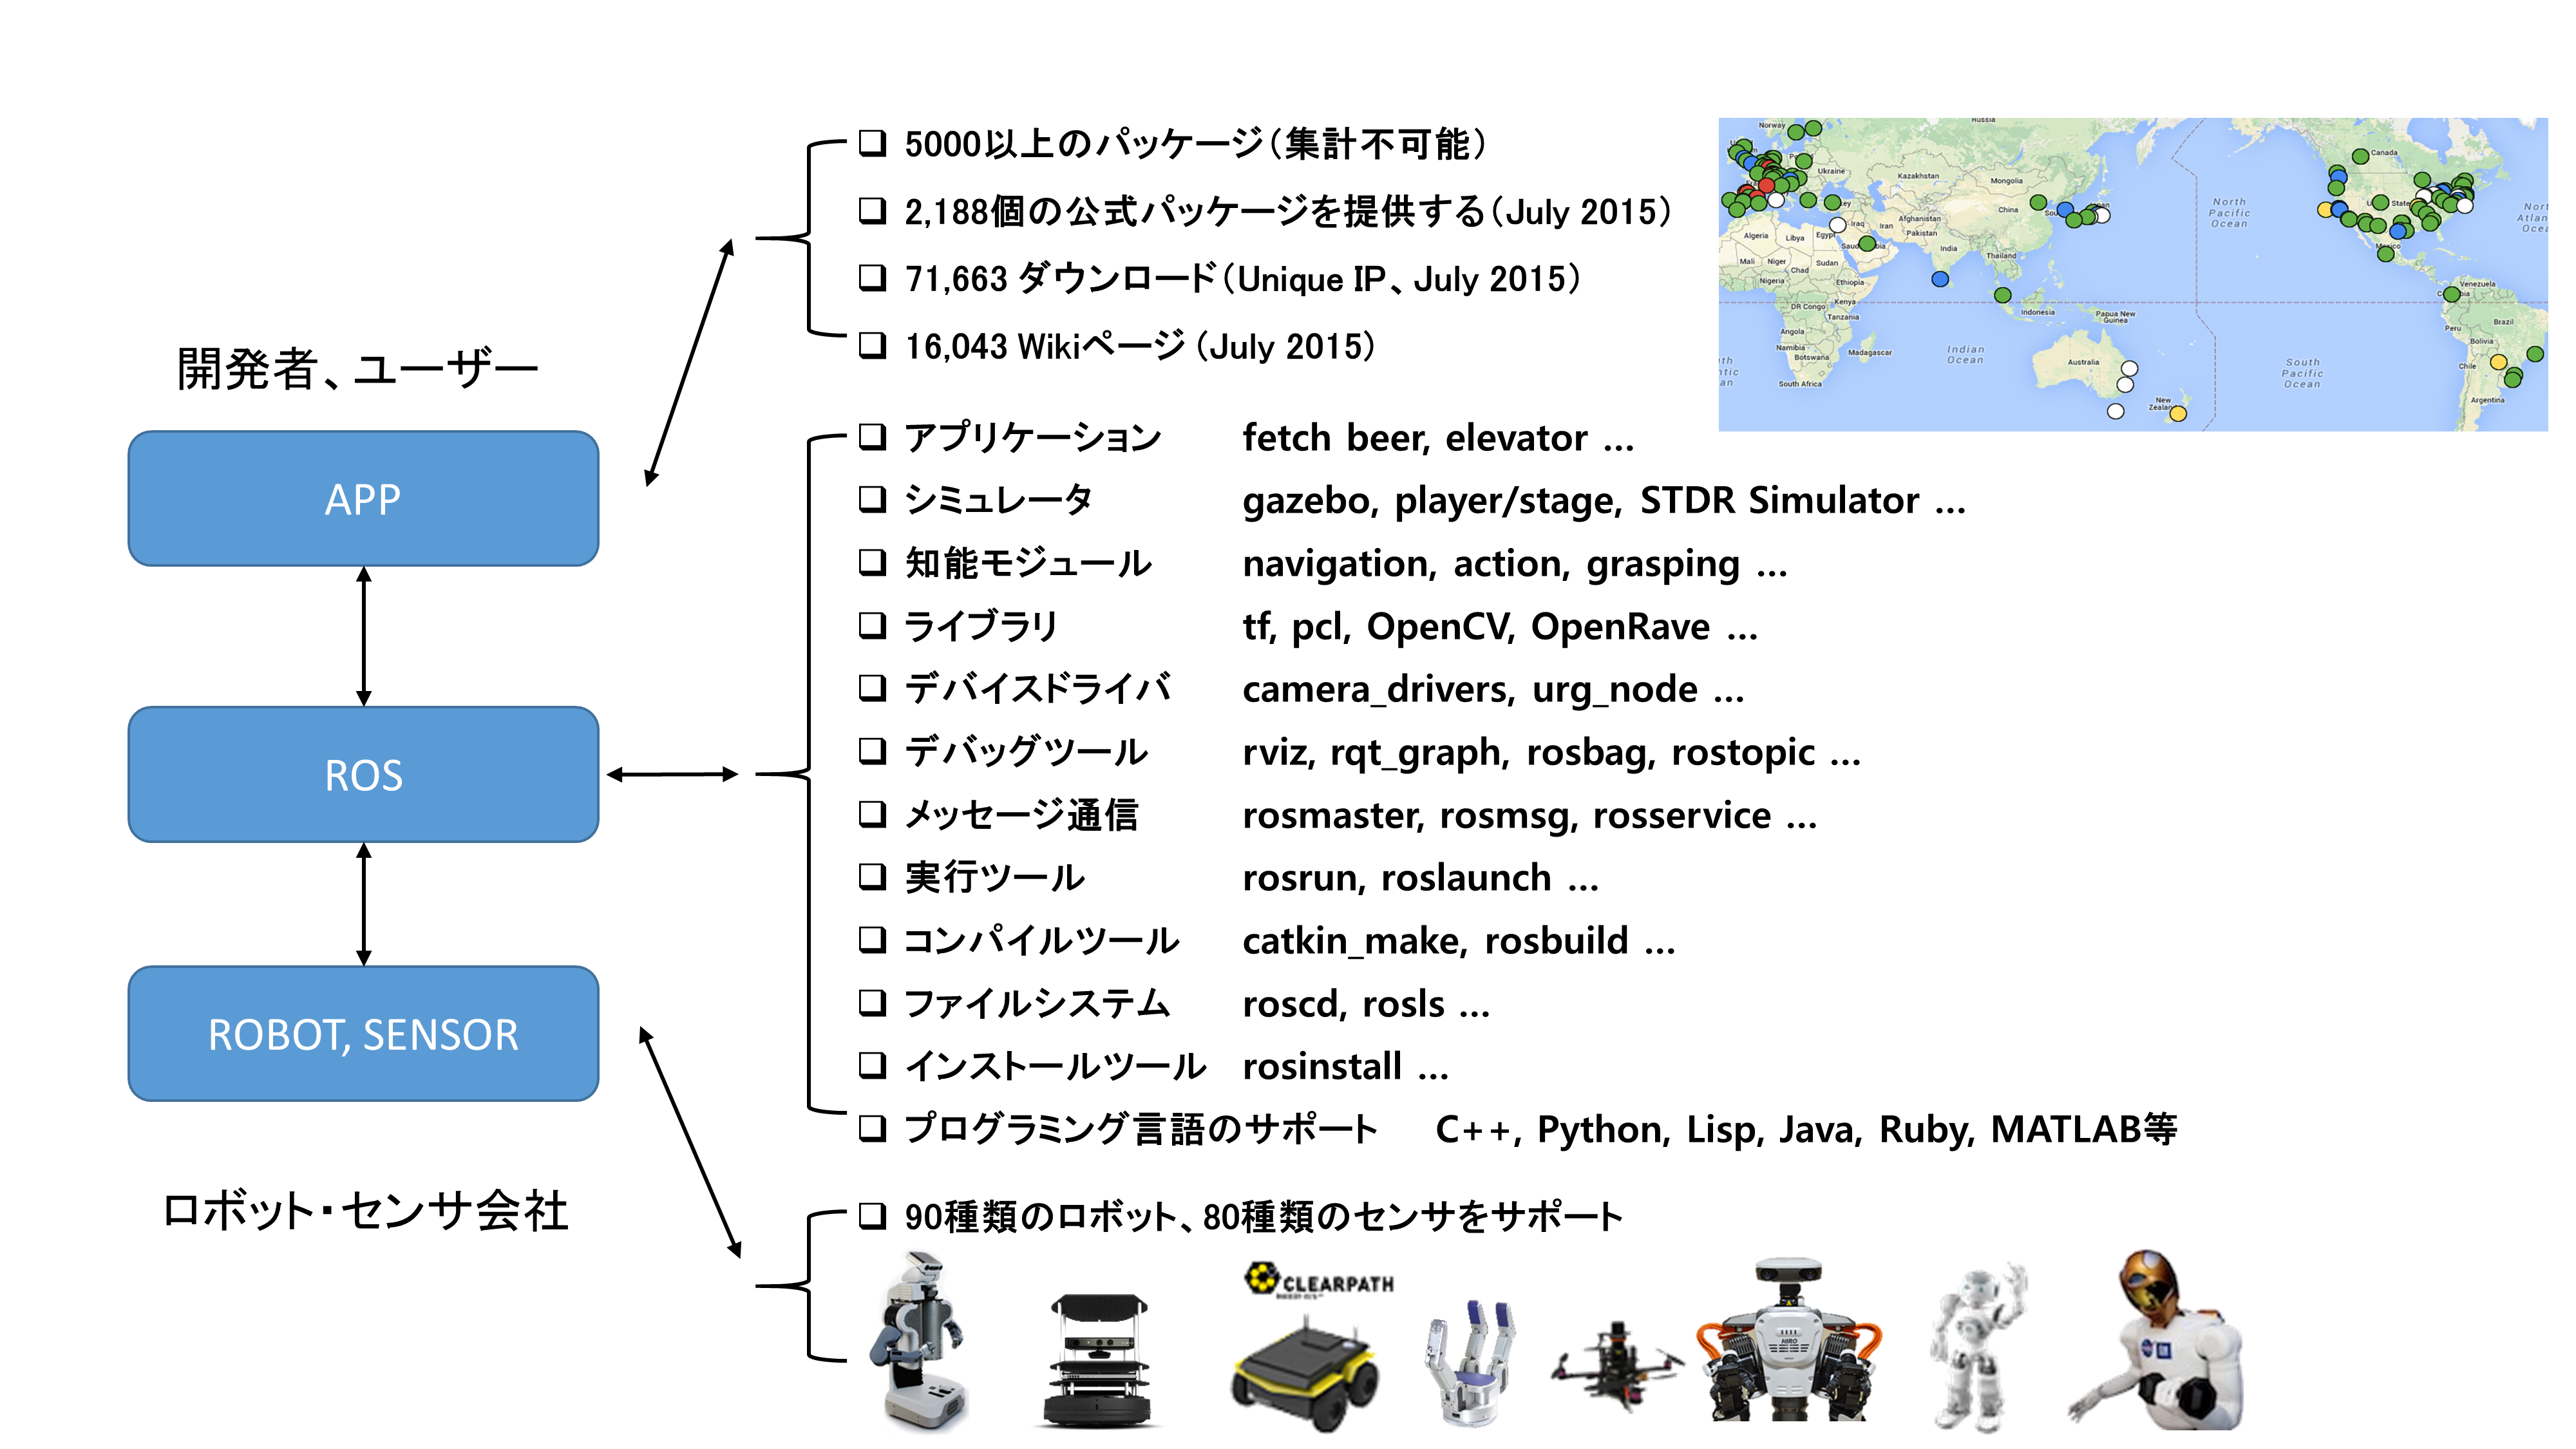
\includegraphics[width=\columnwidth]{pictures/chapter1/pic_01_03.png}
  \caption{ROS生態系}
\end{figure}

図1-3は、ROSCon2015\footnote{\url{http://roscon.ros.org/2015/}}で発表されたROS公式統計\footnote{\url{http://wiki.ros.org/Metrics}}とROS Wikiデータ\footnote{\url{http://www.ros.org/browse/list.php}}\footnote{\url{http://www.ros.org/news/2012/12/ros-five-years.html}}をもとにまとめたROSの現状である。まだ十分とはいえないが、ロボット分野でこれほど広く利用されているロボットソフトウェアプラットフォームは他にはなく、今後も成長が期待されている。

%-------------------------------------------------------------------------------
\section{ROSの歴史}
\index{歴史}\index{History}\index{OSRF}

ROSの技術的な詳細について述べる前に、ROSの歴史を振り返っておこう。 ROSは、2007年5月、米国のスタンフォード大学人工知能研究所(AI LAB)\footnote{\url{http://ai.stanford.edu/}}が実施したSTAIR(STanford AI Robot)プロジェクト\footnote{\url{http://stair.stanford.edu/}}において、Morgan Quigley\footnote{\url{http://www.osrfoundation.org/morgan-quigley.html}}が開発したSwitchyardに端を発する。2007年11月、米国のロボット専門企業Willow GarageがSwitchyardを引き継ぎ、ROSの名前で開発を始めた。Willow Garageは、パーソナルロボットとサービスロボットで著名な企業であり、有名な画像処理オープンソースソフトウエアであるOpenCV\footnote{\url{http://opencv.org/}}や、マイクロソフトKinectなどの3次元計測器で利用されるPCL(Point Cloud Library)\footnote{\url{http://pointclouds.org/}}をサポートしていたことでも知られる。

\begin{figure}[h]
  \centering
  \includegraphics[width=8cm]{pictures/chapter1/pic_01_04.png}
  \caption{ROSロゴ(http://wiki.ros.org/)}
\end{figure}

Willow Garageは、2010年1月22日にROSの開発者向けプレリリース版であるROS 1.0を発表した。その後、2010年3月1日にその公式バージョンであるROS Box Turtleがリリースされた。その後も、C Turtle、Diamondbackなど、UbuntuやAndroidと同様にABC順にバージョン名を付け、アップデートを続けている。 2014年7月にはROSの9番目のバージョンROSインディゴイグルー(Indigo Igloo、公式リリースでは、8番目のバージョン)を公開した。
ROSは、フリーソフトウェアの代表的なライセンス体系であるBSDライセンス(BSD 3-Clause License\footnote{\url{http://opensource.org/licenses/BSD-3-Clause}})をベースにしており、誰でも修正、再利用、再配布が可能である。開発者とユーザーを対象としたカンファレンス(ROSDay、ROSCon)が定期的に開催され、アメリカとヨーロッパではROS Industrial\footnote{\url{http://rosindustrial.org/}} (産業用途のROS)を開発しているコンソーシアムがある。また、それぞれの国で、ROS Meetupと呼ばれるコミュニティが、セミナーなどのイベントを開催している。日本でも、東京オープンソースロボティクス協会(TORK)\footnote{\url{http://opensource-robotics.tokyo.jp/}}やROS JAPAN Users Group\footnote{\url{https://groups.google.com/forum/#!forum/ros-japan-users}}が中心になってセミナーや勉強会を開催し、ROSの普及に努めている。一方、PR2(Personal Robot 2)\footnote{\url{http://www.willowgarage.com/pages/pr2/overview}}やタートルボット(Turtlebot)\footnote{\url{http://turtlebot.com/}}など、ROSの利用を前提としたロボット(リファレンスロボット)の開発も行われている。さらにこれらのリファレンスロボットを利用して多くのアプリケーション開発が行われ、これにより現在ではROSは最も標準的なロボットソフトウェアプラットフォームの一つとなっている。

%-------------------------------------------------------------------------------
\section{ROSのバージョン}
\index{バージョン}\index{Version}\index{Distribution}\index{Indigo Igloo}

Willow GarageがSwitchyardをROS(Robot Operating System)という名前で引き継ぎ、その後7回のバージョンアップを経て、2012年12月にROS Groovy Galapagosバージョンをリリースした。
その後、2013年にWillow Garageが商業サービスロボット市場に参入し、ROSの開発はロボット向けのオープンソースソフトウエア財団であるOSRF(Open Source Robotics Foundation)\footnote{\url{http://osrfoundation.org/}}に移譲された。OSRFは、2014年7月にROSの9番目のバージョンアップROS Indigo Iglooバージョンをリリースした。各リリースは図1-5に示すように亀をモチーフにしたシンボルで表されている。
\\\\
\textbf{ROSのリリース\footnote{\url{http://wiki.ros.org/Distributions}}とカンファレンス\footnote{\url{http://roscon.ros.org/}}}
\begin{itemize}[leftmargin=*]
\item  2016/05/xx: Kinetic \textbf{Kame}リリース予定
\item  2015/10/03: ROSCon2015カンファレンス開催
\item  2015/05/30: Jade Turtleリリース
\item  2014/09/12: ROSCon2014カンファレンス開催
\item  2014/07/22: Indigo Iglooリリース
\item  2014/06/06: ROS Kong 2014開催
\item  2013/09/04: Hydro Medusaリリース
\item  2013/05/11: ROSCon2013カンファレンス開催
\item  2013/02/11: Open Source Robotics Foundationが開発、管理を務める
\item  2012/12/31: Groovy Galapagosリリース
\item  2012/05/19: ROSCon2012カンファレンス開催
\item  2012/04/23: Fuerteリリース
\item  2011/08/30: Electric Emysリリース
\item  2011/03/02: Diamondbackリリース
\item  2010/08/03: C Turtleリリース
\item  2010/03/01: Box Turtleリリース
\item  2010/01/22: ROS 1/0開発
\item  2007/11/01: Willow Garageが「ROS」という名前で開発を開始
\item  2007/05/01: Switchyard、Morgan Quigley、Stanford AI LAB、スタンフォード大学
\item  2000: Player/Stage Project、Brian Gerkey、Richard Vaughan、Andrew Howard、南カリフォルニア大学
\end{itemize}


\begin{figure}[h]
  \centering
  \includegraphics[width=\columnwidth]{pictures/chapter1/pic_01_05.png}
  \caption{ROSのバージョン(http://wiki.ros.org/)}
\end{figure}

%-------------------------------------------------------------------------------
\subsection{ROSのバージョンのルール}
\index{バージョン}\index{Version}

ROSはこれまでに、ROS 1.0、Box Turtle、C Turtle、Diamondback、Electric Emys、Fuerte、Groovy Galapagos、Hydro Medusa、Indigo Igloo、Jade Turtleの10のバージョンをリリースしている。ROSの各バージョンは、2つめのバージョン以降、その頭文字がアルファベット順になるように名づけられている(この命名方式は、UbuntuやAndroidと同様である)。つまり、現在多く使われているIndigo Iglooのバージョンは、アルファベットIバージョン、すなわち9番目のバージョンである。
また、図1-5と図1-6に示すように、各バージョンではポスター形式のイラストと亀のアイコンを発表している。この亀のアイコンは、turtlesim\footnote{\url{http://wiki.ros.org/turtlesim}}というROS公式チュートリアル用のシミュレーションにも使用されている。

\begin{figure}[h]
  \centering
  \includegraphics[width=\columnwidth]{pictures/chapter1/pic_01_06.png}
  \caption{各バージョンの亀のアイコン}
\end{figure}

%-------------------------------------------------------------------------------
\subsection{ROSリリースサイクル}
\index{リリースサイクル}\index{Distributions}\index{LTS}

ROSが正式にサポートしているオペレーティングシステムはUbuntu\footnote{\url{http://www.ubuntu.com/}}であるため、Ubuntuの新バージョンのリリースサイクルと同様に、1年に2回(4月、10月)の更新が行われていた。しかし2013年、ROSの開発と管理を担当しているOSRFは、ユーザーの意見を取り入れて、Hydro Medusaバージョンから1年に1回、Ubuntuの新しいバージョンのリリースに合わせて4月か5月にリリースすることを発表した。
ROSのサポートは、一般的なUbuntuバージョンに合わせたものは1年間、2年に一度リリースされるUbuntu LTS(Long Term Support、例えばUbuntu 14.04)バージョンに合わせたものは、3年間サポートされる。例えば、2014年4月にリリースされたUbuntu 14.04 LTS(Trusty Tahr)に対応するROSのバージョンは、2014年のROS I版と2015年のJ版という2つのバージョンであり、それぞれ2017年4月までサポートされる予定である。現在までのUbuntu向けROSのリリースサイクル\footnote{\url{http://wiki.ros.org/Distributions/Timeline}}は、図1-7のとおりである。\\

\begin{figure}[h]
  \centering
  \includegraphics[width=\columnwidth]{pictures/chapter1/pic_01_07.png}
  \caption{Ubuntu向けROSのリリースサイクル}
\end{figure}

\subsubsection{Ubuntuのリリースサイクルとサポート期間}

Ubuntuは1年で2回、4月と10月にリリースされ、リリース時期によって14.04又は14.10などの名前が付けられている。また、2年間隔の偶数年度は、長期サポート版(Long Term Support)がリリースされる。これは、通常のバージョンが9ヶ月間サポートされるのに対し、LTSサポート期間はリリースから5年間である。LTSは安定した環境を望むユーザーに向いており、ROSユーザーもUbuntu LTSの公開に合わせてバージョンアップすることが多い。

\noindent http://ja.wikipedia.org/wiki/Ubuntu

%-------------------------------------------------------------------------------
\subsection{ROS Indigo Igloo}
\index{Indigo Igloo}

\begin{figure}[h]
  \centering
  \includegraphics[width=8cm]{pictures/chapter1/pic_01_08.png}
  \caption{Indigo Iglooのバージョンのポスターとアイコン}
\end{figure}

現在、ROSのコミュニティで最も使われているバージョンは、2014年7月22日に正式リリースされたROS Indigo Igloo\footnote{\url{http://wiki.ros.org/indigo/}}である。図1-8のようにポスターは、亀がイグルー(ドーム状の家、Igloo)を背負ってスキーを楽しむ姿である。
このバージョンでは、特にcatkin\footnote{\url{http://wiki.ros.org/catkin}}ビルドシステムへの移行に重点を置き、すべてのパッケージがcatkin化された点が特徴的である。それに加え、今回のバージョンからPython3.3への対応や、OpenCVやPCLの標準ライブラリが使用されている。またcmake modulesという名前のパッケージがあり、これに公式サポートしていないパッケージを集約した。さらに、boostのsignal関数をすべてsignal2に変更し、最新のバージョンに対応した。全体的には、マイナーアップグレードとメンテナンスの色合いが強い。

%-------------------------------------------------------------------------------
\subsection{ROSのバージョンの選択}
\index{バージョン}\index{Version}\index{Release}\index{Ubuntu}\index{LTS}\index{Indigo Igloo}
\label{section:rosversion}

ROSはメタ・オペレーティングシステムであり、ROSを利用するには、まず基本的に使用するオペレーティングシステムを選択する必要がある。ROSはUbuntu、Mac OS X、Fedora、Gentoo、OpenSUSE、Debian、Arch Linux、Windowsなどの多くのオペレーティングシステムをサポートしているが、ROSのユーザーが最も多く使用しているオペレーティングシステムはUbuntuである。開発チームでもUbuntuのLTSバージョン\footnote{\url{https://wiki.ubuntu.com/Releases}}に合わせて新バージョンをリリースしていることから、特に支障がない限り、UbuntuのLTSバージョンに合ったROSのバージョンを選択することが好ましい。
ROSの各バージョンにおけるUbuntuの対応状況に関する情報は、関連ROS Wikiサイトである「http://www.ros.org/debbuild/」にアクセスし、使用予定のROSのバージョンを選択することで得られる。このファイルには、現在選択しているROSのバージョンに対し、Ubuntuのバージョンごとに、既存のROSパッケージに対する最新のROSのバージョンへの対応状況が記載されている。例えば、「http://www.ros.org/debbuild/indigo.html」では、図1-9のようにIndigo Iglooのバージョンの対応状況が確認できる。内容はパッケージの名前(Name)、パッケージのレポジトリ(Repo)、バージョン(Version)、開発やメンテナンスされているかの情報(Wet Status)、メインテナー(Maintainer)、各UbuntuとROSのバージョンに対する移植状況等が記載されている。特に移植状況には注意する必要があるので、図1-10を例に説明する。

\begin{figure}[h]
  \centering
  \includegraphics[width=\columnwidth]{pictures/chapter1/pic_01_09.png}
  \caption{Indigo Iglooのバージョンの移植状況}
\end{figure}

\begin{figure}[h]
  \centering
  \includegraphics[width=\columnwidth]{pictures/chapter1/pic_01_10.png}
  \caption{Indigo Iglooのバージョンの移植状況の詳細}
\end{figure}

① IsrcS:ROS Indigo(I)バージョンのソース(src)のUbuntu 13.10 Saucy(S)バージョンに対する情報である。また、「IbinT64」の場合は、ROS Indigo(I)バージョンのバイナリ(bin)、64ビット Ubuntu 14.04 Trusty Tahr(T64)バージョンを意味する。
②、③、④ :色付きの四角のアイコンは、building, shadow-fixed, ros/publicを意味する。buildingは開発側のビルド状況、shadow-fixedは公式に出る直前のテストのためのレポジトリで、ros/publicは公式リリースされたレポジトリを示す。各色は、緑が問題なく移植された場合、青が以前のバージョンのままの場合、赤が移植できなかった場合、黄色が今回のバージョンに移植できないか、今後は使用しない場合、灰色は意図的に外したものである。
⑤ 番号:1744、1744、1692などは、それぞれbuilding, shadow-fixed, ros/publicで使えるパッケージの数を意味する。
ROSの最新バージョンへの移行を考える際、まず自分が使用したいパッケージがROSやUbuntuのバージョンに対応済みかを確認する必要がある。ROSの最新バージョンでは、多くのパッケージが「移植中」と表示されるが、使用したいパッケージ、および重要なパッケージが対応済みであれば最新バージョンに移行しても構わない。一方、もし使用したいパッケージが最新バージョンに対応していない場合には、移行は見合わせるべきである。
\\
\begin{itemize}
\item Ubuntu 15.10: Wily Werewolf
\item Ubuntu 15.04: Vivid Vervet
\item Ubuntu 14.10: Utopic Unicorn
\item \textbf{Ubuntu 14.04: Trusty Tahr(LTS)}
\item Ubuntu 13.10: Saucy Salamander
\item Ubuntu 13.04: Raring Ringtail
\item Ubuntu 12.10: Quantal Quetzal
\item Ubuntu 12.04: Precise Pangolin(LTS)
\item Ubuntu 11.10: Oneiric Ocelot
\item Ubuntu 11.04: Natty Narwhal
\item Ubuntu 10.10: Maverick Meerkat
\item Ubuntu 10.04: Lucid Lynx(LTS)
\end{itemize}
\\
本書では、2016年に次のUbuntu LTSバージョンがリリースされるまでは、以下の組み合わせを推奨する。

\begin{itemize}
\item オペレーティングシステム:\textbf{Ubuntu 14.04 Trusty Tahr(LTS)}
\item ROSのバージョン:\textbf{ROS Indigo Igloo}
\end{itemize}

%-------------------------------------------------------------------------------
